\documentclass[10pt]{beamer}
\usetheme[
%%% options passed to the outer theme
%    hidetitle,           % hide the (short) title in the sidebar
%    hideauthor,          % hide the (short) author in the sidebar
%    hideinstitute,       % hide the (short) institute in the bottom of the sidebar
%    shownavsym,          % show the navigation symbols
%    width=2cm,           % width of the sidebar (default is 2 cm)
%    hideothersubsections,% hide all subsections but the subsections in the current section
%    hideallsubsections,  % hide all subsections
    left               % right of left position of sidebar (default is right)
%%% options passed to the color theme
%    lightheaderbg,       % use a light header background
  ]{AAUsidebar}

% If you want to change the colors of the various elements in the theme, edit and uncomment the following lines
% Change the bar and sidebar colors:
%\setbeamercolor{AAUsidebar}{fg=red!20,bg=red}
%\setbeamercolor{sidebar}{bg=red!20}
% Change the color of the structural elements:
%\setbeamercolor{structure}{fg=red}
% Change the frame title text color:
%\setbeamercolor{frametitle}{fg=blue}
% Change the normal text color background:
%\setbeamercolor{normal text}{bg=gray!10}
% ... and you can of course change a lot more - see the beamer user manual.


\usepackage[utf8]{inputenc}
\usepackage[english]{babel}
\usepackage[T1]{fontenc}
% Or whatever. Note that the encoding and the font should match. If T1
% does not look nice, try deleting the line with the fontenc.
\usepackage{helvet}

%Custom packages
\usepackage{graphicx}
\graphicspath{{graphics/}}

% colored hyperlinks
\newcommand{\chref}[2]{%
  \href{#1}{{\usebeamercolor[bg]{AAUsidebar}#2}}%
}

\title[Decentralized Label Model]% optional, use only with long paper titles
{A Decentralized Model for Information Flow Control}

\subtitle{Andrew C. Myers and Barbara Liskov, 1997}  % could also be a conference name

\date{September 23, 2015}

\author[Mikael Elki\ae r Christensen] % optional, use only with lots of authors
{
  Mikael Elki\ae r Christensen\\
  \href{mailto:michri11@student.aau.dk}{{\tt michri11@student.aau.dk}}
}
% - Give the names in the same order as they appear in the paper.
% - Use the \inst{?} command only if the authors have different
%   affiliation. See the beamer manual for an example

\institute[
%  {\includegraphics[scale=0.2]{aau_segl}}\\ %insert a company, department or university logo
  Department of Computer Science\\
  Aalborg University\\
  Denmark
] % optional - is placed in the bottom of the sidebar on every slide
{% is placed on the title page
  Department of Computer Science\\
  Aalborg University\\
  Denmark
  
  %there must be an empty line above this line - otherwise some unwanted space is added between the university and the country (I do not know why;( )
}


% specify a logo on the titlepage (you can specify additional logos an include them in 
% institute command below
\pgfdeclareimage[height=1.5cm]{titlepagelogo}{AAUgraphics/aau_logo_new} % placed on the title page
%\pgfdeclareimage[height=1.5cm]{titlepagelogo2}{graphics/aau_logo_new} % placed on the title page
\titlegraphic{% is placed on the bottom of the title page
  \pgfuseimage{titlepagelogo}
%  \hspace{1cm}\pgfuseimage{titlepagelogo2}\textsl{}
}


\begin{document}
% the titlepage
{\aauwavesbg%
\begin{frame}[plain,noframenumbering] % the plain option removes the sidebar and header from the title page
  \titlepage
\end{frame}}
%%%%%%%%%%%%%%%%

%% TOC
%\begin{frame}{Agenda}{}
%\tableofcontents
%\end{frame}
%%%%%%%%%%%%%%%%

\section{Introduction}
\begin{frame}{Introduction}{}
The result of this paper is a model for controlling information flow: \alert{Decentralized Label Model (DLM)}.
\end{frame}
%%%%%%%%%%%%%%%%

\subsection{What it is not}
\begin{frame}{Introduction}{What it is not}
	\only<1->{It is not:}
	\begin{itemize}
		\item <2-> Access Control
		\item <3-> Authentication, Authorization, Confidentiality, Integrity.
	\end{itemize}
	
	\only<4->{This means that DLM will \alert{not} ensure:}
	\begin{itemize}
		\item <5-> secure communication between applications
		\item <6-> limited access to data once released
	\end{itemize}
\end{frame}
%%%%%%%%%%%%%%%%

\subsection{What it is}
\begin{frame}{Introduction}{What it is}
	\only<1->{It is:}
	\begin{itemize}
		\item <2-> Information Flow Control
		\item <3-> Decentralized
	\end{itemize}
	\only<4->{This means that DLM will help ensuring:}
	\begin{itemize}
		\item <5-> not releasing sensitive data
		\item <6-> not implicitly releasing sensitive data
		\item <7-> not giving away hints of inner workings
	\end{itemize}
\end{frame}
%%%%%%%%%%%%%%%%

\subsection{How it differs}
\begin{frame}{Introduction}{How it differs}
	\only<1->{DLM differs from previous solutions as it is:}
	\begin{itemize}
		\item <2-> decentralized
		\item <3-> less restrictive of allowed computations
		\item <4-> not completely disallowing inter-application communication
		\item <5-> meant to extend current programming languages with data flow annotations
	\end{itemize}
\end{frame}
%%%%%%%%%%%%%%%%

\section{DLM Basics}
\begin{frame}{DLM Basics}{}
	DLM provides both static and dynamic checking of data flow.
\end{frame}
%%%%%%%%%%%%%%%%\textsl{}

\subsection{Terminology}
\begin{frame}{DLM Basics}{Terminology}
	\begin{description}
		\item <1-> [Principals] represent users and other authoritative entities (e.g. groups or roles).
		\item <2-> [Values] are entities computations can manipulate.
		\item <3-> [Slots] are value-holders (e.g. variables, objects, and other storage locations).
		\item <4-> [Input channels] are read-only sources that allow information to enter the system.
		\item <5-> [Output channels] are information sinks that transmit information outside the system.
		\item <6-> [Labels] are attached to values, slots or channels (more to follow).
	\end{description}
\end{frame}
%%%%%%%%%%%%%%%%

\subsection{Labels}
\begin{frame}{DLM Basics}{Labels}
	\only<1->{A label $\mathbf{L}$ is a set of owners, where each owner denotes its readers, e.g.:
	\[ \{ o_1 : r_1, r_2; o_2 : r_2, r_3 \} \]
	where $o_1, o_2, r_1, r_2, r_3$ are principals.}
	\\[0.25cm]
	\only<2->{The effective reader set of a label is the intersection of every reader, for $\mathbf{L}$ it is $\{r_2\}$.}
\end{frame}
%%%%%%%%%%%%%%%%

\subsection{Key Principles}
\begin{frame}{DLM Basics}{Key Principles}
	\begin{itemize}
		\item <1-> Labels are comparable:
		\begin{itemize}
			\item <1-> $\mathbf{L_1} \sqsubseteq \mathbf{L_2}$ signifies that $\mathbf{L_2}$ is at least as restrictive as $\mathbf{L_1}$.
		\end{itemize}
		\item <2-> Labels can be joined:
		\begin{itemize}
			\item <2-> $\mathbf{L_1} \sqcup \mathbf{L_2}$ results in a join of owners and intersection of readers.
		\end{itemize}
		\item <3-> Principals can act for other principals.
		\item <4-> Relabeling can be done, further restricting or declassifying.
	\end{itemize}
\end{frame}
%%%%%%%%%%%%%%%%

\section{Example}
\begin{frame}{Example}{}
	\centering
	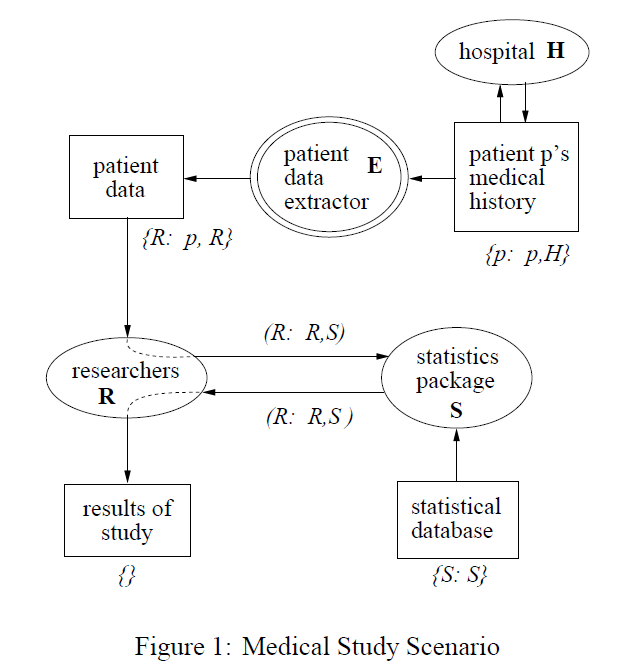
\includegraphics[height=.7\paperheight]{hospital_example.png}
\end{frame}
%%%%%%%%%%%%%%%%

\subsection{Code Example}
\begin{frame}{Example}{Code Example}
	\centering
	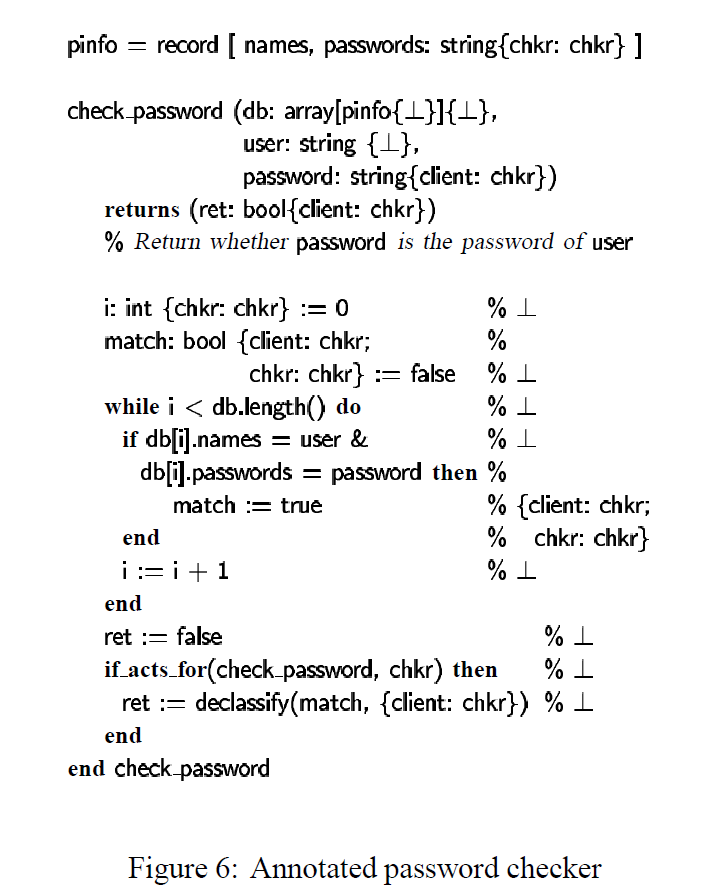
\includegraphics[height=.7\paperheight]{passwordcheker_example.png}
\end{frame}
%%%%%%%%%%%%%%%%

\section{Advanced}
\begin{frame}{Advanced}{}
	\begin{itemize}
		\item Label polymorphism
		\item Run-time labels (\texttt{lb} type)
		\item Protected types (\texttt{protected[T]})
		\item Inferred labels
	\end{itemize}
\end{frame}
%%%%%%%%%%%%%%%%

\section{Conclusion}
\begin{frame}{Conclusion}{}
	\begin{itemize}
		\item <1-> Decentralized Label Model
		\item <2-> Control of information flow
		\item <3-> Static and dynamic label checking
		\item <4-> Possible to extend existing programming languages
	\end{itemize}
\end{frame}
%%%%%%%%%%%%%%%%

\subsection{Future Works}
\begin{frame}{Conclusion}{Future Works}
	\begin{itemize}
		\item <1-> Actual implementation (JIF -- dead)
		\item <2-> Support for user-defined data abstractions
		\item <3-> Formal proofs
		\item <4-> Network systems
		\item <5-> Threading
	\end{itemize}
\end{frame}
%%%%%%%%%%%%%%%%

{\aauwavesbg
\begin{frame}[plain,noframenumbering]
  \finalpage{Questions?}
\end{frame}}
%%%%%%%%%%%%%%%%

\end{document}
